% VISUAL-MANAGED-FILE
% Curated Q&A appendix. Internal process, retired estimates, and open-test dashboards are intentionally excluded.

% VISUAL-FUNCTION: appendix coverage | categorized navigation map | route audience questions to defensible evidence
\begin{frame}{Appendix map}
\begin{columns}[T]
\begin{column}{0.47\textwidth}
\textbf{Definitions and data}
\begin{itemize}
\item A1 Route units and vehicle status
\item A2 Asset types and backing regimes
\item A3 Sample construction and exclusions
\end{itemize}
\vspace{0.45cm}
\textbf{Reconstruction and validation}
\begin{itemize}
\item A4 Exact transaction state
\item A5 Protocol-specific state
\item A6 Forced routes in V1
\end{itemize}
\end{column}
\begin{column}{0.47\textwidth}
\textbf{Robustness}
\begin{itemize}
\item A7 Daily and weekly frequencies
\item A8 Count and value weighting
\item A9 Endpoint demand
\end{itemize}
\vspace{0.45cm}
\textbf{Mechanisms}
\begin{itemize}
\item A10 Capital, inventory, and depth
\item A11 Coordination and integration
\item A12--A13 References
\end{itemize}
\end{column}
\end{columns}
\end{frame}

% VISUAL-FUNCTION: route counting unit | one-path transaction glyph | distinguish route units from swap legs
\begin{frame}{A1. One reconstructed route is one unit}
\begin{columns}[T]
\begin{column}{0.47\textwidth}
\centering
\begin{tikzpicture}
\node[nodepoint] (a) at (0,1.6) {$i$};
\node[nodepoint,fill=ucldark,text=white,draw=ucldark] (k) at (2.0,1.6) {$k$};
\node[nodepoint] (b) at (4.0,1.6) {$o$};
\draw[route] (a)--(k);
\draw[route] (k)--(b);
\node[font=\small\bfseries] at (2.0,0.55) {one route unit};
\node[font=\small] at (2.0,0.05) {two swap legs};
\end{tikzpicture}
\end{column}
\begin{column}{0.47\textwidth}
\begin{itemize}
\item Each linked $i\rightarrow k\rightarrow o$ route is counted once.
\item Asset $k$ is classified as the intermediary on that route.
\item Dominance is the share of route units or supported value carried by $k$.
\end{itemize}
\end{column}
\end{columns}
\end{frame}

% VISUAL-FUNCTION: time-varying asset types | regime taxonomy pending token-period heatmap | make heterogeneity contemporaneous rather than fixed
\begin{frame}{A2. Backing regimes vary over time}
\begin{columns}[T]
\begin{column}{0.47\textwidth}
\textbf{Native platform asset}\par ETH, WETH; volatile settlement asset and protocol-native demand.
\vspace{0.45cm}
\textbf{Fiat-reserve stablecoin}\par USDC, USDT; reserve and redemption design.
\end{column}
\begin{column}{0.47\textwidth}
\textbf{On-chain collateralised}\par DAI, LUSD, crvUSD; collateral, liquidation, and backing changes.
\vspace{0.45cm}
\textbf{Tokenised external asset}\par WBTC, tokenised gold; wrapped claim on an external asset.
\end{column}
\end{columns}
\vspace{0.75cm}
{\small Heterogeneity tests use each asset's contemporaneous backing regime.\par}
\end{frame}

% VISUAL-FUNCTION: primary measurement funnel | staged route-object and two-support split | separate topology support from dollar-value support
% EVIDENCE-STATUS: qualitative measurement contract; no attrition quantities shown.
% EVIDENCE-COMMIT: 2ffbce06302468b5ee6cb6537989c28078a88603
% EVIDENCE-SOURCES: deck/assets/sample-measurement-funnel.tex;
% docs/specification-lock.json; docs/findings-freeze.md;
% data/manifests/data/processed/intermediation_by_type_daily.parquet.prov.json.
\begin{frame}{A3. One route universe supports two measurements}
\centering
\resizebox{0.96\textwidth}{!}{% VISUAL-MANAGED-ASSET
% VISUAL-FUNCTION: primary measurement funnel | staged route-object and two-support split | separate topology support from dollar-value support
% EVIDENCE-STATUS: qualitative measurement contract; box widths do not encode sample size.
% EVIDENCE-COMMIT: 2ffbce06302468b5ee6cb6537989c28078a88603
% EVIDENCE-SOURCES: docs/specification-lock.json; docs/findings-freeze.md;
% data/manifests/data/processed/intermediation_by_type_daily.parquet.prov.json.
% INPUT-SHA256: 8db2065d8f14b8a3d7b34b6cc2057823a6d74ecc5fc8f8b6beaef33c7afc780b
\begin{tikzpicture}[
  x=1cm,
  y=1cm,
  stage/.style={rounded corners=2pt,draw=rule,fill=panel,minimum width=2.18cm,
    minimum height=1.18cm,text width=1.88cm,align=center,inner sep=4pt,font=\scriptsize},
  countlane/.style={rounded corners=2pt,draw=native,fill=native!7,minimum width=4.10cm,
    minimum height=0.94cm,text width=3.72cm,align=center,inner sep=4pt,font=\scriptsize},
  valuelane/.style={rounded corners=2pt,draw=stable,fill=stable!7,minimum width=4.10cm,
    minimum height=0.94cm,text width=3.72cm,align=center,inner sep=4pt,font=\scriptsize}
]
\node[stage] (legs) at (0,0) {released\\swap legs};
\node[stage] (routes) at (2.75,0) {reconstructed\\economic routes};
\node[stage] (twoleg) at (5.50,0) {exact two-leg\\intermediary routes};
\node[stage,draw=ucldark,line width=1pt] (choice) at (8.25,0) {native--stable\\choice set};

\draw[route,draw=muted] (legs)--node[above=17pt,font=\tiny,text=muted,align=center] {link legs into\\one route} (routes);
\draw[route,draw=muted] (routes)--node[above=17pt,font=\tiny,text=muted,align=center] {remove endpoint\\round trips} (twoleg);
\draw[route,draw=muted] (twoleg)--node[above=17pt,font=\tiny,text=muted,align=center] {classify the\\intermediary} (choice);

\node[countlane] (count) at (3.40,-2.03) {\textbf{Route-count evidence}\quad one qualifying route, one vote};
\node[valuelane] (value) at (7.93,-2.03) {\textbf{Strict-value evidence}\quad both leg values agree within 20\%};

\draw[-{Stealth[length=5pt]},line width=1.25pt,draw=native]
  (choice.south west) .. controls (7.30,-0.88) and (5.20,-1.00) .. (count.north);
\draw[-{Stealth[length=5pt]},line width=1.25pt,draw=stable]
  (choice.south east) .. controls (8.86,-0.88) and (8.35,-1.08) .. (value.north);

\node[font=\tiny,text=muted,align=center] at (5.50,-3.04)
  {Topology-valid routes remain in count evidence when dollar support is unavailable.\\Box widths do not represent attrition.};
\end{tikzpicture}
}\par
\vspace{0.12cm}
{\small Missing dollar support narrows value-weighted evidence; it does not erase a topology-valid route from the count evidence.\par}
\end{frame}

% VISUAL-FUNCTION: causal event ordering | numbered replay sequence | explain same-state counterfactual timing
\begin{frame}{A4. State is reconstructed immediately before execution}
\begin{tikzpicture}[x=1cm,y=1cm]
\node[softbox,text width=2.10cm,minimum height=1.35cm,align=center] (checkpoint) at (0,0) {\textbf{1}\\verified starting state};
\node[softbox,text width=2.10cm,minimum height=1.35cm,align=center] (events) at (3.20,0) {\textbf{2}\\apply events in blockchain order};
\node[softbox,text width=2.10cm,minimum height=1.35cm,align=center] (pre) at (6.40,0) {\textbf{3}\\recover state before the trade};
\node[softbox,text width=2.10cm,minimum height=1.35cm,align=center,draw=ucldark] (quote) at (9.60,0) {\textbf{4}\\quote both routes};
\draw[route] (checkpoint)--(events);
\draw[route] (events)--(pre);
\draw[route] (pre)--(quote);
\end{tikzpicture}
\vspace{0.85cm}
\begin{itemize}
\item Pool events are applied in blockchain order from a verified starting state.
\item Each route is quoted using the pool state immediately before the transaction.
\item Missing state intervals are excluded, and their share of trading volume is reported.
\end{itemize}
\end{frame}

% VISUAL-FUNCTION: protocol-specific state requirements | protocol-by-state matrix | prevent false comparability across AMM families
% Source contract: docs/research-workflow.md lines 161--163 and 382--384;
% src/ddvc/execution_contracts.py and src/ddvc/liquidity.py at f16d5f074fac73011dce1c609d80146ec3fd3bec.
% Filled squares mean that the field enters the family-specific pre-trade state;
% the outlined V4 hook square records an explicit perimeter restriction, not measured hook state.
\begin{frame}{A5. Each AMM family has a different state vector}
\begin{center}
\setlength{\tabcolsep}{4.7pt}
\renewcommand{\arraystretch}{1.55}
\scriptsize
\begin{tabular}{@{}p{2.80cm}ccccccc@{}}
\toprule
& \shortstack{reserves or\\active liquidity}
& ticks
& amplification
& \shortstack{weights or\\scaling}
& \shortstack{rates or\\oracles}
& fees
& hooks \\
\midrule
Constant product
& {\color{native}$\blacksquare$} & -- & -- & -- & -- & {\color{native}$\blacksquare$} & -- \\
Concentrated liquidity
& {\color{uclbright}$\blacksquare$} & {\color{uclbright}$\blacksquare$} & -- & -- & -- & {\color{uclbright}$\blacksquare$} & -- \\
StableSwap families
& {\color{stable}$\blacksquare$} & -- & {\color{stable}$\blacksquare$} & -- & {\color{stable}$\blacksquare$} & {\color{stable}$\blacksquare$} & -- \\
Weighted pools
& {\color{imported}$\blacksquare$} & -- & -- & {\color{imported}$\blacksquare$} & {\color{imported}$\blacksquare$} & {\color{imported}$\blacksquare$} & -- \\
V4 singleton
& {\color{accent}$\blacksquare$} & {\color{accent}$\blacksquare$} & -- & -- & -- & {\color{accent}$\blacksquare$} & {\color{accent}$\square$} \\
\bottomrule
\end{tabular}
\end{center}
\vspace{0.25cm}
\begin{columns}[T]
\begin{column}{0.68\textwidth}
{\small The common object is the state immediately before execution. The fields required to recover that state vary with the pricing rule.\par}
\end{column}
\begin{column}{0.27\textwidth}
{\scriptsize\color{muted}{\color{ink}$\blacksquare$} required state\\[0.25em]{\color{accent}$\square$} hooks outside comparison\par}
\end{column}
\end{columns}
\end{frame}

% VISUAL-FUNCTION: compulsory V1 intermediation | two-leg trace pending authentic transaction rows | establish imposed ETH routing from observables
\begin{frame}{A6. V1 forced routes have an on-chain signature}
\begin{columns}[T]
\begin{column}{0.43\textwidth}
\begin{itemize}
\item Token-to-token execution emits two linked swaps through ETH.
\item Matching ETH quantities distinguish protocol-imposed intermediation from unrelated bundled swaps.
\end{itemize}
\end{column}
\begin{column}{0.53\textwidth}
\centering
\begin{tikzpicture}[scale=1.0,transform shape]
\node[nodepoint] (a) at (0,0) {$i$};
\node[nodepoint,fill=ucldark,text=white,draw=ucldark,minimum size=30pt] (e) at (2.5,0) {ETH};
\node[nodepoint] (b) at (5.0,0) {$o$};
\draw[route,draw=accent] (a)--node[above,font=\small] {$x$ ETH} (e);
\draw[route,draw=accent] (e)--node[above,font=\small] {$x$ ETH} (b);
\node[font=\small\bfseries,text=ucldark,align=center] at (2.5,-1.55) {same transaction, matching ETH flow};
\end{tikzpicture}
\end{column}
\end{columns}
\end{frame}

% VISUAL-FUNCTION: observation and response clocks | list pending exact-horizon diagram | separate aggregation from elapsed-time links
\begin{frame}{A7. Daily and weekly frequencies answer different questions}
\begin{enumerate}
\item \textbf{Primary panel}\hfill day observations; date fixed effects
\item \textbf{Calendar sensitivity}\hfill day observations; week and weekday fixed effects
\item \textbf{Aggregation robustness}\hfill complete weeks; week fixed effects
\item \textbf{Transition series}\hfill exact 1-, 7-, 30-, and 120-day links; HAC inference
\end{enumerate}
\vspace{0.65cm}
{\small Weekly ratios are formed from weekly sums; results are reported for weeks ending on each day of the week.\par}
\end{frame}

% VISUAL-FUNCTION: route weights | paired formulas pending equal-versus-value-width routes | distinguish frequency from economic scale
\begin{frame}{A8. Count and value define separate dominance margins}
\begin{columns}[T]
\begin{column}{0.46\textwidth}
\textbf{Count-weighted share}
\[
S^{N}_{k,t}=\frac{N^I_{k,t}}{\sum_j N^I_{j,t}}
\]
Each reconstructed route carries one unit of weight.
\end{column}
\begin{column}{0.46\textwidth}
\textbf{Value-weighted share}
\[
S^{V}_{k,t}=\frac{\mathrm{Vol}^I_{k,t}}{\sum_j \mathrm{Vol}^I_{j,t}}
\]
Each route carries reliably priced dollar value on common support.
\end{column}
\end{columns}
\vspace{0.75cm}
{\small Differences between count and value shares may reflect trade size, route structure, or the mix of intermediary assets.\par}
\end{frame}

% VISUAL-FUNCTION: intermediary excess use | paired margin formulas pending zero-centered difference plot | separate vehicle demand from endpoint demand
\begin{frame}{A9. Endpoint demand and intermediary use are separate margins}
\begin{columns}[T]
\begin{column}{0.46\textwidth}
\textbf{Intermediary share}
\[
S^I_{k,t}=\frac{N^I_{k,t}}{\sum_j N^I_{j,t}}
\]
How often asset $k$ sits inside a route.
\end{column}
\begin{column}{0.46\textwidth}
\textbf{Endpoint share}
\[
S^E_{k,t}=\frac{N^{\mathrm{in}}_{k,t}+N^{\mathrm{out}}_{k,t}}{\sum_j N^{\mathrm{in}}_{j,t}+N^{\mathrm{out}}_{j,t}}
\]
How often asset $k$ is what traders buy or sell.
\end{column}
\end{columns}
\vspace{0.55cm}
{\large\color{ucldark}\bfseries Excess use compares intermediation with endpoint demand on the same support.\par}
\end{frame}

% VISUAL-FUNCTION: liquidity quantities | labelled pool-state and price-response cross-section | prevent capital, inventory, depth, and quote quality from collapsing
% EVIDENCE-STATUS: conceptual institutional background; no empirical estimate.
% EVIDENCE-COMMIT: 525c67a7f672593fe07e54cf5ccb6d08910e9b04
% EVIDENCE-SOURCES: deck/assets/liquidity-quantity-cross-section.tex;
% src/ddvc/liquidity.py; src/ddvc/capital_contracts.py.
\begin{frame}{A10. Capital, inventory, and depth are different objects}
\centering
\resizebox{0.965\textwidth}{!}{% EVIDENCE-STATUS: conceptual institutional diagram; contains no empirical estimate.
% EVIDENCE-SOURCES: src/ddvc/liquidity.py; src/ddvc/capital_contracts.py;
% README.md (capital, inventory, depth, and quote semantics).
% The generic price-response curve deliberately avoids imposing one AMM invariant.
\tikzset{callout/.style={rounded corners=2pt,draw=rule,fill=panel,inner sep=5pt,align=center,font=\scriptsize}}
\tikzset{poolbin/.style={rounded corners=3pt,draw=ucldark,line width=1.1pt,fill=white,minimum width=2.10cm,minimum height=1.18cm,align=center}}
\tikzset{guide/.style={draw=muted,densely dashed,line width=0.8pt}}
\begin{tikzpicture}[x=1cm,y=1cm]

% Balance-sheet view: claims and token holdings are different objects.
\node[font=\small\bfseries,text=ucldark,anchor=west] at (0.0,3.18) {Pool balance sheet at time $t$};
\node[callout,minimum width=2.05cm] (lp) at (0.90,2.48) {LP positions\\or audited claims};
\node[poolbin] (x) at (0.95,0.95) {$R_{X,p,t}$ units\\of token $X$};
\node[poolbin] (y) at (3.42,0.95) {$R_{Y,p,t}$ units\\of token $Y$};
\draw[route,draw=uclbright] (lp.south) -- ++(0,-0.40) -| (x.north);
\draw[route,draw=uclbright] (lp.south) -- ++(0,-0.40) -| (y.north);
\node[font=\scriptsize\bfseries,text=ink] at (2.18,-0.04) {inventory: exact token holdings};
\draw[decorate,decoration={brace,mirror,amplitude=5pt},draw=stable,line width=1pt]
  (-0.14,0.26) -- (4.52,0.26);
\node[callout,minimum width=3.40cm,anchor=north] at (2.18,-0.24)
  {deposited capital: independently valued holdings\\or validated ownership claims};

% Execution view: a trade size maps through current state into depth and a quote.
\draw[rule,line width=0.8pt] (5.35,0.10) -- (5.35,3.05);
\node[font=\small\bfseries,text=ucldark,anchor=west] at (5.85,3.18) {Execution from that state};
\draw[-{Stealth[length=4pt]},draw=ink,line width=0.9pt] (6.05,0.48) -- (11.45,0.48)
  node[below left,font=\scriptsize] {input size};
\draw[-{Stealth[length=4pt]},draw=ink,line width=0.9pt] (6.05,0.48) -- (6.05,2.82);
\node[font=\scriptsize,rotate=90] at (5.72,1.66) {price impact};
\draw[draw=ucldark,line width=1.7pt]
  (6.15,0.68) .. controls (8.05,0.82) and (9.50,1.42) .. (11.15,2.65);
\fill[native] (7.12,0.87) circle (2.6pt);
\fill[accent] (9.92,1.76) circle (2.6pt);
\draw[guide] (7.12,0.48) -- (7.12,0.87);
\draw[guide] (9.92,0.48) -- (9.92,1.76);
\draw[<->,draw=stable,line width=1.2pt] (7.12,0.27) -- node[below,font=\scriptsize,text=stable] {$q$} (9.92,0.27);
\draw[<->,draw=accent,line width=1.2pt] (10.17,0.87) -- (10.17,1.76);
\path[fill=stable,opacity=0.12] (7.12,0.48) -- (7.12,0.87) .. controls (8.30,1.00) and (9.08,1.34) .. (9.92,1.76) -- (9.92,0.48) -- cycle;
\node[callout,draw=stable,anchor=north,minimum width=3.25cm] at (8.46,-0.02)
  {executable depth: quantity available\\within a stated price-impact band};
\node[callout,draw=accent,anchor=west,minimum width=1.58cm] at (10.40,1.58)
  {quote quality\\at size $q$};

\end{tikzpicture}
}\par
\vspace{0.12cm}
{\small Capital is a stock. Depth and quotes depend on trade size and current pool state.\par}
\end{frame}

% VISUAL-FUNCTION: opportunity set versus realised composition | multiplex network and route-class small multiples | separate feasible paths from selected routes
% EVIDENCE-STATUS: conceptual institutional background; no empirical estimate.
% EVIDENCE-COMMIT: 525c67a7f672593fe07e54cf5ccb6d08910e9b04
% EVIDENCE-SOURCES: deck/assets/integration-multiplex-network.tex;
% docs/research-workflow.md; docs/specification-lock.json.
\begin{frame}{A11. Integration changes the routes that can be chosen}
\centering
\resizebox{0.94\textwidth}{!}{% EVIDENCE-STATUS: conceptual institutional diagram; contains no empirical estimate.
% EVIDENCE-COMMIT: 525c67a7f672593fe07e54cf5ccb6d08910e9b04
% EVIDENCE-SOURCES: docs/research-workflow.md (integration and route-class semantics);
% docs/specification-lock.json (routing_maturation_e0 and vehicle_transition_e0).
% Venue names and route classes are generic; the diagram makes no adoption or causal claim.
\begin{tikzpicture}[x=1cm,y=1cm,
  asset/.style={circle,draw=ink,fill=white,minimum size=19pt,inner sep=0pt,font=\scriptsize},
  venue/.style={rounded corners=4pt,draw=rule,fill=panel,minimum width=4.55cm,minimum height=1.36cm},
  routecard/.style={rounded corners=3pt,draw=rule,fill=white,minimum width=4.15cm,minimum height=1.08cm},
  faintpath/.style={-{Stealth[length=4pt]},draw=muted,line width=0.85pt},
  chosenpath/.style={-{Stealth[length=4pt]},draw=ucldark,line width=1.5pt}]

\node[font=\small\bfseries,text=ucldark,anchor=west] at (0.0,3.25) {Feasible venue layers};

% Two venue layers form the opportunity set.
\node[venue] (va) at (2.32,2.20) {};
\node[font=\scriptsize\bfseries,text=native,anchor=west] at (0.18,2.70) {venue $a$};
\node[asset] (ia) at (0.78,2.15) {$i$};
\node[asset,fill=ucldark,text=white,draw=ucldark] (ka) at (2.32,2.15) {$k$};
\node[asset] (oa) at (3.86,2.15) {$o$};
\draw[faintpath] (ia)--(ka);
\draw[faintpath] (ka)--(oa);
\draw[faintpath,draw=stable] (ia) to[bend left=28] (oa);

\node[venue] (vb) at (2.32,0.54) {};
\node[font=\scriptsize\bfseries,text=uclbright,anchor=west] at (0.18,1.04) {venue $b$};
\node[asset] (ib) at (0.78,0.49) {$i$};
\node[asset,fill=ucldark,text=white,draw=ucldark] (kb) at (2.32,0.49) {$k$};
\node[asset] (ob) at (3.86,0.49) {$o$};
\draw[faintpath] (ib)--(kb);
\draw[faintpath] (kb)--(ob);
\draw[faintpath,draw=stable] (ib) to[bend right=28] (ob);

\draw[draw=rule,densely dashed] (ia)--(ib);
\draw[draw=rule,densely dashed] (ka)--(kb);
\draw[draw=rule,densely dashed] (oa)--(ob);
\node[font=\scriptsize,text=muted,align=center] at (2.32,-0.38) {venue layers share assets;\\available links define reach};

% Conditioning arrow, deliberately not a causal arrow.
\draw[-{Stealth[length=6pt]},draw=uclbright,line width=1.4pt] (4.92,1.35) -- (6.15,1.35);
\node[font=\scriptsize,text=muted,align=center] at (5.54,1.82) {realised\\execution};

% Route-class outcomes on the right.
\node[font=\small\bfseries,text=ucldark,anchor=west] at (6.35,3.25) {Realised route topology};

\node[routecard] at (8.55,2.46) {};
\node[font=\scriptsize\bfseries,anchor=west] at (6.62,2.82) {direct};
\node[asset] (d1) at (7.75,2.26) {$i$};
\node[asset] (d2) at (9.56,2.26) {$o$};
\draw[chosenpath,draw=stable] (d1)--(d2);

\node[routecard] at (8.55,1.22) {};
\node[font=\scriptsize\bfseries,anchor=west] at (6.62,1.58) {sequential intermediary};
\node[asset] (s1) at (7.70,0.99) {$i$};
\node[asset,fill=ucldark,text=white,draw=ucldark] (sk) at (8.76,0.99) {$k$};
\node[asset] (s2) at (9.82,0.99) {$o$};
\draw[chosenpath,draw=native] (s1)--node[above,font=\tiny] {$a$} (sk);
\draw[chosenpath,draw=uclbright] (sk)--node[above,font=\tiny] {$b$} (s2);

\node[routecard] at (8.55,-0.02) {};
\node[font=\scriptsize\bfseries,anchor=west] at (6.62,0.34) {split direct};
\node[asset] (p1) at (7.75,-0.25) {$i$};
\node[asset] (p2) at (9.56,-0.25) {$o$};
\draw[chosenpath,draw=native] (p1) to[bend left=24] node[above,font=\tiny] {$a$} (p2);
\draw[chosenpath,draw=uclbright] (p1) to[bend right=24] node[below,font=\tiny] {$b$} (p2);

\end{tikzpicture}
}\par
\vspace{0.10cm}
{\small The analysis therefore separates opportunity-set reach from the composition of realised routes.\par}
\end{frame}

% VISUAL-FUNCTION: realised venue scope by intermediary type | count/value alluvial | show that integration and vehicle composition are distinct observed margins
% EVIDENCE-STATUS: evolving route composition; descriptive selected-route cross-section.
% EVIDENCE-COMMIT: 2ffbce06302468b5ee6cb6537989c28078a88603
% EVIDENCE-SOURCES: output/figures/experiments/integration_vehicle_alluvial.pdf;
% output/exhibits/intermediation_by_type.jsonl; docs/reviews/deck-visual-experiments.md.
% INPUT-SHA256: 539a9feb5712a899cc901023eea8e62f56bf6015a23af8c6e735e981b874e12a
\begin{frame}{A11b. Venue scope and vehicle type differ in 2026}
\vfill
\begin{center}
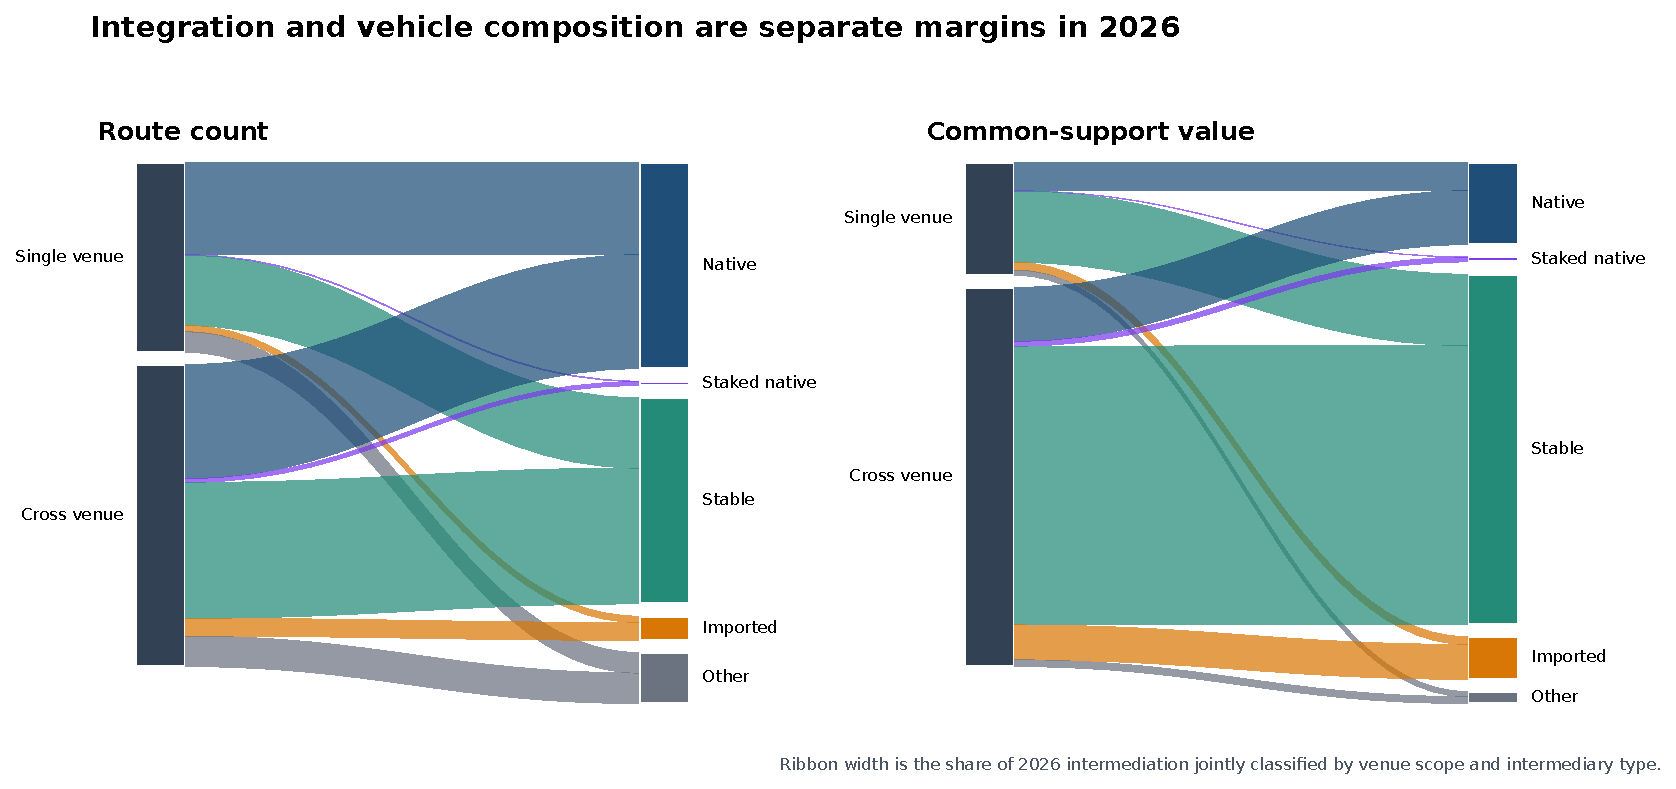
\includegraphics[width=0.93\textwidth,height=0.66\textheight,keepaspectratio]{../output/figures/experiments/integration_vehicle_alluvial.pdf}
\end{center}
\vspace{-0.12cm}
{\scriptsize The ribbons classify realised intermediation jointly by venue scope and intermediary type. They describe selected routes; they do not identify an effect of integration or the unchosen opportunity set.\par}
\vfill
\end{frame}

% VISUAL-FUNCTION: intellectual provenance | grouped reference list | support vehicle-currency and market-structure framing
\begin{frame}{A12. References: vehicle currencies and market structure}
\begin{itemize}
\item Amiti, Itskhoki and Konings (2022), \emph{Quarterly Journal of Economics}
\item Dowd and Greenaway (1993), \emph{Economic Journal}
\item Flandreau and Jobst (2009), \emph{Economic Journal}
\item Gopinath and Stein (2021), \emph{Quarterly Journal of Economics}
\item Krugman (1980), \emph{Journal of Money, Credit and Banking}
\item Makarov and Schoar (2020), \emph{Journal of Financial Economics}
\end{itemize}
\end{frame}

% VISUAL-FUNCTION: institutional provenance | grouped reference list | support AMM architecture and liquidity design
\begin{frame}{A13. References: decentralised exchange design}
\begin{itemize}
\item Adams et al. (2021), \emph{Uniswap v3 Core}
\item Angeris, Chitra, Evans and Boyd, optimal routing in constant-function markets
\item Barbon and Ranaldo, decentralised exchange costs and market structure
\item Lehar and Parlour (2024), \emph{Journal of Finance}
\item Milionis, Moallemi, Roughgarden and Zhang, loss versus rebalancing
\item Xu, Paruch, Cousaert and Feng, AMM design and slippage
\end{itemize}
\end{frame}
